\label{sec:demo}
%%%%%%%%%%%%%%%%%%%%%%%%
In order to show the capabilities introduced with the new Adaptive DET module, a simplified PWR Dynamic PRA analysis is here presented.
Figure~\ref{fig:PWRmodel} shows the scheme of the PWR model. The reactor vessel model consists of the down-comers, the lower plenum, the reactor core model, and the upper plenum. core channels (flow channels with heat structure attached to each of them) are used to describe the reactor core. The core model consists of three parallel core channels and one bypass flow channel. There are two primary loops, i.e., loop A and loop B. Each loop consists of hot leg, heat exchanger and secondary side pipes, cold leg, and primary pump. A pressurizer is attached to the loop A piping system to control system pressure. A time dependent volume (pressure boundary conditions) component is used to represent the pressurizer. Since the RELAP-7 code two-phase flow capability has not been used for this test, single-phase counter-current heat exchanger models are implemented to mimic the function of steam generators to transfer heat from the primary to the secondary.

The DPRA analysis of this simplified model here presented, it has been performed by controlling unconventional parameters to speed up the simulation and overcome some modeling challenges. In the following paragraph, the PRA station black out sequence of events is reported.
\begin{figure}[h]
   \centering
    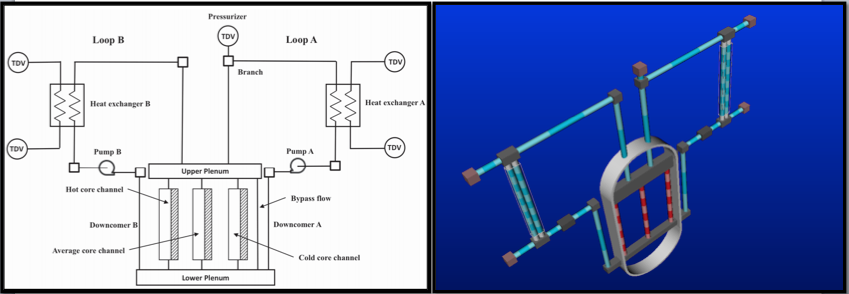
\includegraphics[width=1.0\textwidth]{figures/PWR_TMI_SCHEME.PNG}
    \caption{PWR model scheme}
    \label{fig:PWRmodel}
\end{figure}
%%%%%%%%%%%%%%%%%%%%%%%%%%%%%%
\subsection{Station Black Out (SBO) analysis} 
%%%%%%%%%%%%%%%%%%%%%%%%%%%%%%
\label{sec:SBOanalysis}
The simulation of a SBO initiating event required the introduction, in the control logic, of several components (see Fig.~\ref{fig:SchemeElSystem}):
\begin{figure}[h]
   \centering
    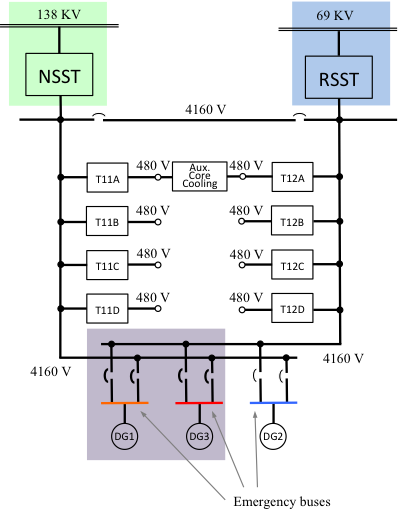
\includegraphics[width=0.4\textwidth]{figures/SchemeEletricalSystem.png}
    \caption{Scheme of the electrical system of the PWR model}
    \label{fig:SchemeElSystem}
\end{figure}

\begin{itemize}
\item Set of 3 diesel generators (DGs) and associated emergency buses
\item Primary power grid line 138 KV (connected to the NSST switchyard)
\item Auxiliary power grid line 69 KV (connected to the RSST switchyard)
\item Electrical buses: 4160 V (step down voltage from the power grid and voltage of the electric converter connected to the DGs) and 480 V for actual reactor components (e.g., reactor cooling system)
\end{itemize}
The scenario is as follows:
\begin{itemize}
\item An external event (e.g. earthquake, etc.) causes a Loss Of Off-site Power (LOOP) due to damage of the 138 kV line and RSST switchyard; the reactor successfully scrams and, thus, thermal energy generated in the core follows the characteristic exponential decay curve
\item The set of DGs fails to start up and, hence, conditions of SBO are reached (4160 V and 480 V buses are not energized); all auxiliary cooling systems are subsequently off-line, and therefore the removal of decay heat from the reactor core is not ensured
\item Without the ability to cool the reactor core, its temperature starts to rise
\item In order to recover AC electric power on the 4160 V and 480 V buses, two recovery teams are assembled with the following strategy:
\begin{itemize}
\item Recovery Team 1 focuses on the recovery of the DGs: due to internal damage at the DG building, two DGs (i.e., DG1 and DG3) need to be repaired (see Fig.~\ref{fig:ACPowerRecovery}~(a))
\item Recovery Team 2 focuses on the recovery of the RSST switchyard; 69KV line is energized but the RSST switchyard needs to be recovered (see Fig.~\ref{fig:ACPowerRecovery}~(b))
\end{itemize}
\item Meanwhile the utility company is working on the restoration of the primary 138 KV line (see Fig.~\ref{fig:ACPowerRecovery}~(c))
\item When the 4160 V buses are energized (through the recovery of the DGs, RSST or 138KV line), the auxiliary cooling system is able to cool the reactor core and, thus, core temperature decreases
\end{itemize}

\begin{figure}
        \centering %
        ~ %add desired spacing between images, e. g. ~, \quad, \qquad etc.
          %(or a blank line to force the subfigure onto a new line)
        \begin{subfigure}[b]{0.3\textwidth}
                \centering
                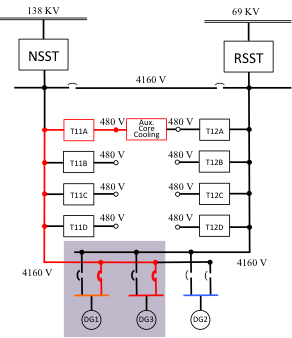
\includegraphics[width=\textwidth]{figures/ACpowerRecPathDGs.png}
                \caption{}
                \label{fig:ACpowerDGs}
        \end{subfigure}
        \begin{subfigure}[b]{0.3\textwidth}
                \centering
                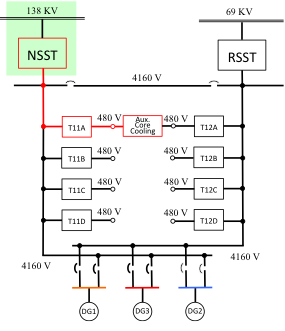
\includegraphics[width=\textwidth]{figures/ACpowerRecPath138kV.png}
                \caption{}
                \label{fig:ACpower138kV}
        \end{subfigure}
        ~ %add desired spacing between images, e. g. ~, \quad, \qquad etc.
          %(or a blank line to force the subfigure onto a new line)
        \begin{subfigure}[b]{0.3\textwidth}
                \centering
                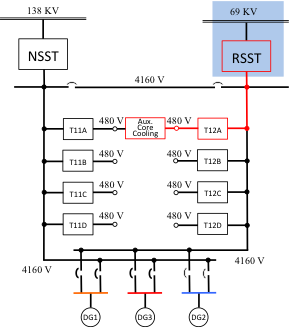
\includegraphics[width=\textwidth]{figures/ACpowerRecPathRSST.png}
                \caption{}
                \label{fig:ACpowerRSST}
        \end{subfigure}
        \caption{AC power recovery paths through: DGs (a), RSST (b) and 138KV line (c). Red lines indicate electrical path to power Auxiliary cooling system}\label{fig:ACPowerRecovery}
\end{figure}

Given the uncertainties associated to the recovery timing of DGs, RSST and 138KV line, a probabilistic model has been employed to represent these events. The corresponding probability distribution functions are as follows:
\begin{itemize}
\item DGs: a dead time of 100s is required by Team 1 to reach the DGs building and DGs' repair time $TDG$ has a normal distribution having mu = 800 and sigma = 200. This distribution is also truncated such that $0 < TDG1 < 2500$
\item RSST: a dead time of 400s is needed to assess the damage at the RSST switch-yard and to organize its recovery. Recovery time for RSST, TRSST , is normally distributed with mu = 1400 and sigma= 400
\item 138KV line: the recovery of the main AC line T138 is normally distributed with mu = 2000 and sigma = 500
\end{itemize}

In addition, the clad failure temperature $T_{C,fail}$, our success/failure criterion, is probabilistic distributed with a triangular distribution with the following characteristics:
\begin{itemize}
\item mode(apex): 1477.59 K, 10CFR regulatory limit
\item lower bound: 1255.37 K, PRA success criterion
\item upper bound: 1699.82 K, Urbanic-Heidrick transition temperature ~\cite{Urbanic1978}
\end{itemize}

%%%%%%%%%%%%%%%%%%%%%%%%%%%%%%
The PRA analysis for this accident scenario has been carried over using the ADET algorithm. The parameters controlling the convergence of the iterative process has been chosen such as the maximum error in terms of the determination of the probability of failure of the system would be below 1.0E-4.

As already mentioned, the ADET methodology performs a pre-screening of the input space through a standard DET approach, before starting the real adaptive scheme. In this specific case, pre-screening DET calculation has been run using equally spaced branching probability thresholds for all uncertain parameters considered in this scenario.

\begin{figure}
        \centering %
        ~ %add desired spacing between images, e. g. ~, \quad, \qquad etc.
          %(or a blank line to force the subfigure onto a new line)
        \begin{subfigure}[b]{0.48\textwidth}
                \centering
                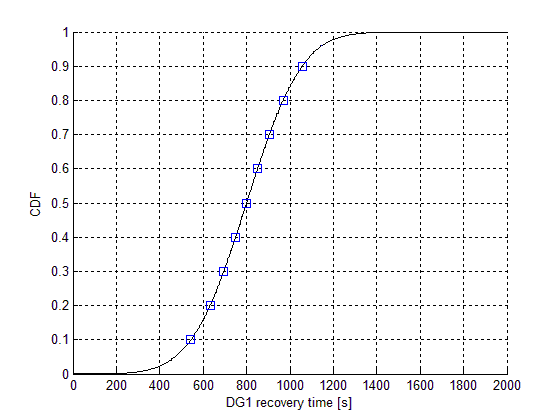
\includegraphics[width=\textwidth]{figures/DG1Dist.png}
                \caption{}
                \label{fig:DG1Dist}
        \end{subfigure}
%        \begin{subfigure}[b]{0.48\textwidth}
%               \centering
%                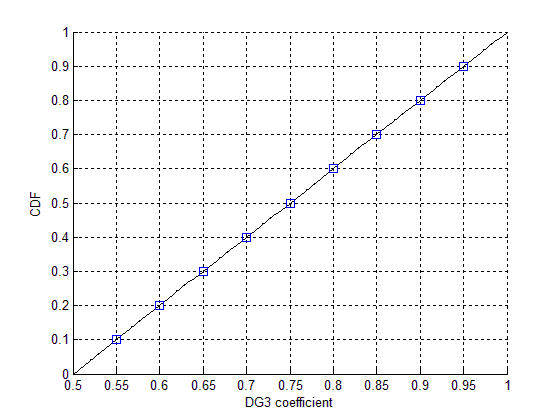
\includegraphics[width=\textwidth]{figures/DG3CoeffDist.png}
%                \caption{}
%                \label{fig:DG3CoeffDist}
%        \end{subfigure}
        ~ %add desired spacing between images, e. g. ~, \quad, \qquad etc.
          %(or a blank line to force the subfigure onto a new line)
        \caption{Cumulative Distribution Functions and DET bins  for DGs}\label{fig:CDFsDGs}
\end{figure}
\begin{figure}
        \centering %
        ~ %add desired spacing between images, e. g. ~, \quad, \qquad etc.
          %(or a blank line to force the subfigure onto a new line)
        \begin{subfigure}[b]{0.48\textwidth}
                \centering
                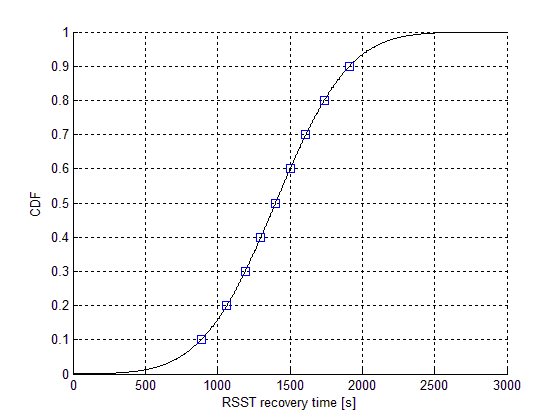
\includegraphics[width=\textwidth]{figures/RSSTDist.png}
                \caption{}
                \label{fig:RSSTDist}
        \end{subfigure}
        \begin{subfigure}[b]{0.48\textwidth}
                \centering
                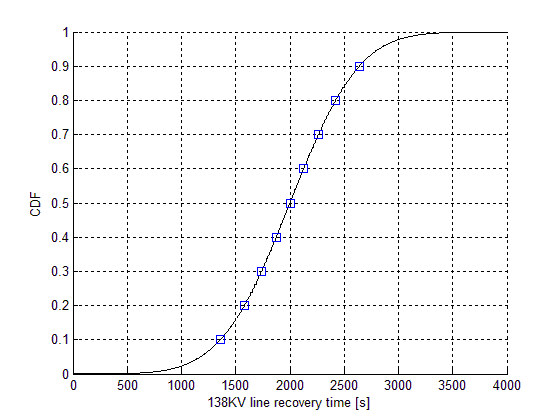
\includegraphics[width=\textwidth]{figures/138kVlineDist.png}
                \caption{}
                \label{fig:138kVlineDist}
        \end{subfigure}
        ~ %add desired spacing between images, e. g. ~, \quad, \qquad etc.
          %(or a blank line to force the subfigure onto a new line)
        \caption{Cumulative Distribution Functions and DET bins: (a) 138kV line, (b) RSST}\label{fig:CDFsACs}
\end{figure}
\begin{figure}
        \centering %
        ~ %add desired spacing between images, e. g. ~, \quad, \qquad etc.
          %(or a blank line to force the subfigure onto a new line)
        \begin{subfigure}[b]{0.48\textwidth}
                \centering
                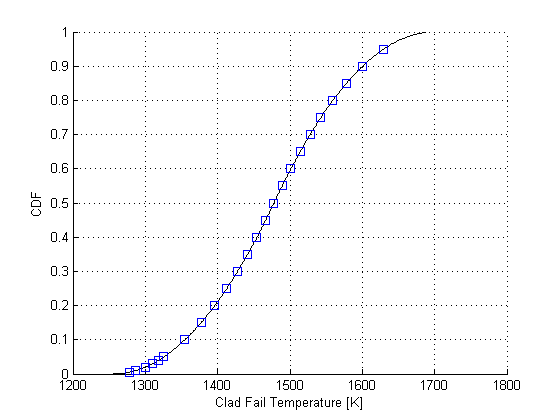
\includegraphics[width=\textwidth]{figures/CladFailureDist.png}
                \caption{}
                \label{fig:CladFailure}
        \end{subfigure}
        \caption{Cumulative Distribution Function and DET bin for Clad Failure Temperature Distribution}\label{fig:CDFCladFailure}
\end{figure}
The probability threshold values are reported below:
\vspace{-5mm}
   \begin{itemize}
       \item DGs' recovery time distribution (Fig.~\ref{fig:CDFsDGs}~(a) - blue points): 
       \begin{itemize} 
            \item Probability Thresholds: 0.1, 0.2, 0.3, 0.4, 0.5, 0.6, 0.7, 0.8,  0.9
            \item Variable Values (s)           : 543.69 , 631.68, 695.12, 749.33, 800.00, 850.67, 904.88, 968.32, 1056.31
       \end{itemize}
       \item RSST recovery time distribution (Fig.~\ref{fig:CDFsACs}~(a) - blue points): 
       \begin{itemize} 
            \item Probability Thresholds:  0.1, 0.2,  0.3,  0.4, 0.5, 0.6, 0.7,  0.8,  0.9
            \item Variable Values (s)           :  887.38, 1063.35, 1190.24, 1298.66, 1400.00, 1501.34, 1609.76, 1736.65, 1912.62
       \end{itemize}
       \item 138 kV line recovery time distribution (Fig.~\ref{fig:CDFsACs}~(b) - blue points): 
       \begin{itemize} 
            \item Probability Thresholds: 0.1, 0.2, 0.3, 0.4, 0.5, 0.6, 0.7, 0.8, 0.9 
            \item Variable Values (s)           : 1359.22,  1579.19,  1737.80, 1873.33,  2000.00,  2126.67, 2262.20,  2420.81, 2640.78
       \end{itemize}
       \item Clad Failure Temperature distribution (Fig.~\ref{fig:CDFCladFailure} - blue points): 
       \begin{itemize} 
            \item Probability Thresholds: 0.005, 0.01, 0.02, 0.03, 0.04, 0.05, 0.10, 0.15, 0.2, 0.25, 0.3, 0.35, 0.4, 0.45, 0.5, 0.55, 0.60, 0.65, 0.70, 0.75, 0.80, 0.85, 0.90, 0.95
            \item Variable Values (K)           : 1304.57, 1307.51, 1313.27, 1318.89, 1324.38, 1329.37, 1354.78, 1376.74, 1395.86, 1412.68, 1427.70, 1441.33, 1453.96, 1465.94, 1477.60, 1489.26, 1501.24, 1513.87, 1527.50, 	1542.51, 1559.34, 1578.45, 1600.40, 1625.79
    \end{itemize}
\end{itemize}
\vspace{-5mm}

In the following section, the simulations results are shown and discussed.
%%%%%%%%%%%%%%%%%%%%%%%%%%%%%%
\subsection{Results} 
%%%%%%%%%%%%%%%%%%%%%%%%%%%%%%
In order to show the newer capability added in RAVEN code, a standard DET~\cite{alfonsiPSA,DETmilestone2013} analysis analysis and an Adaptive tree (ADET) have been compared. 

Figure~\ref{fig:SampledTEMP} shows histograms of the “sampled” clad failure temperatures for DET and ADET. It can be noticed how the Adaptive DET (right figure) focuses on the higher temperatures, reasonably closer to failure regions. The standard DET (left figure) presents a spike in the histogram for the lowest temperatures. This is due to the intrinsic initial mechanics of the methodology in the exploration of the input space (in this case, no branches on clad failure temperature until the first transition is reached).

As already mentioned, the cooling of the system is ensured when:
\begin{itemize}
\item Diesel Generators are repaired, or,
\item the 138 kV line is restored, or, 
\item the RSST switch-yard is repaired. 
\end{itemize}
\begin{table}[h]
\begin{tabular}{|c|c|c|c|c|
>{\columncolor[HTML]{FFCCC9}}c |}
\hline
                                                                        & \textbf{\begin{tabular}[c]{@{}c@{}}Clad Temp\\ Failure\end{tabular}} & \textbf{\begin{tabular}[c]{@{}c@{}}DGS\\ Recovery Time\end{tabular}} & \textbf{\begin{tabular}[c]{@{}c@{}}SecPG\\ Recovery Time\end{tabular}} & \textbf{\begin{tabular}[c]{@{}c@{}}PrimPG\\ Recovery Time\end{tabular}} & \textbf{\begin{tabular}[c]{@{}c@{}}Clad\\ Damaged\end{tabular}} \\ \hline
\textbf{\begin{tabular}[c]{@{}c@{}}Clad Temp \\ Failure\end{tabular}}   & 1.00E+00                                                             & -5.99E-18                                                            & -9.66E-19                                                              & -1.31E-17                                                               & -2.78E-01                                                       \\ \hline
\textbf{\begin{tabular}[c]{@{}c@{}}DGS\\ Recovery Time\end{tabular}}    & -5.99E-18                                                            & 1.00E+00                                                             & 3.56E-17                                                               & 3.56E-18                                                                & 3.20E-01                                                        \\ \hline
\textbf{\begin{tabular}[c]{@{}c@{}}SecPG\\ Recovery Time\end{tabular}}  & -9.66E-19                                                            & 3.56E-17                                                             & 1.00E+00                                                               & -2.37E-18                                                               & 1.60E-02                                                        \\ \hline
\textbf{\begin{tabular}[c]{@{}c@{}}PrimPG\\ Recovery Time\end{tabular}} & -1.31E-17                                                            & 3.56E-18                                                             & -2.37E-18                                                              & 1.00E+00                                                                & 2.38E-01                                                        \\ \hline
\textbf{\begin{tabular}[c]{@{}c@{}}Clad\\ Damaged\end{tabular}}         & -2.78E-01                                                            & 3.20E-01                                                             & 1.60E-02                                                               & 2.38E-01                                                                & 1.00E+00                                                        \\ \hline
\end{tabular}
\caption{Pearson Correlation Matrix.}
\label{table:corr}
\end{table}
Such a situation determines that the timing of these events can be pratically collapsed into a global recovery time of the cooling system. This helps us in the 2-Dimensional visualization of the results (ACS recovery time vs. clad failure temperature). Figure~\ref{fig:SampledCollapsed} shows the sampled points (translated in collapsed time) for the DET (left picture) and ADET (right figure) methodologies. It can be seen how both methodologies march toward higher recovery times, looking for the first transition that determines the first branch for the Clad Failure temperature. Obviously, the ADET method starts its adaptive strategy in proximity to the clad failure transitions, which is the goal function transition surface.

Figure~\ref{fig:LS_DETADET} shows the limit surface obtained by the ADET. As expected, the LS testifies that the higher is the clad failure temperature, the more time we can wait before recovering the auxiliary cooling systems.  The LS for the DET is not shown here, as it is extremely similar to the one just seen.
Table~\ref{table:corr} shows the correlation coefficients' matrix.  As is shown in  the last column, the failure of the clad is inversely proportional to the clad failure temperature. This means, as expected, increasing its threshold reduces the probability of failure of the system. The correlation coefficients of the other parameters (timing of recovery of the cooling system) are instead all positive; meaning the probability of failure increases if those parameters increase. Since the transient, subject of this analysis, is quite fast, obviously the DGs recovery time is the most important (mean = 800 seconds) and the recovery of the 138 kV power line is of lesser importance (mean = 2,000 seconds). As for the LS, the DET correlation matrix is not show here, since it does not add any different information.

For both approaches, the probability of failure has been computed. The ADET and DET methods determined a probability of failure of $0.277 \pm 0.229$ and $0.227\pm 0.402$, respectively. Since the Adaptive methodology is much more focused on the failure regions, its sigma is consequently lower.
%%%%%%%%%%%%%%%
%%% SAMPLED TEMPERATURE
\begin{figure}[h]
 \begin{minipage}[b]{8.5cm}
   \centering
   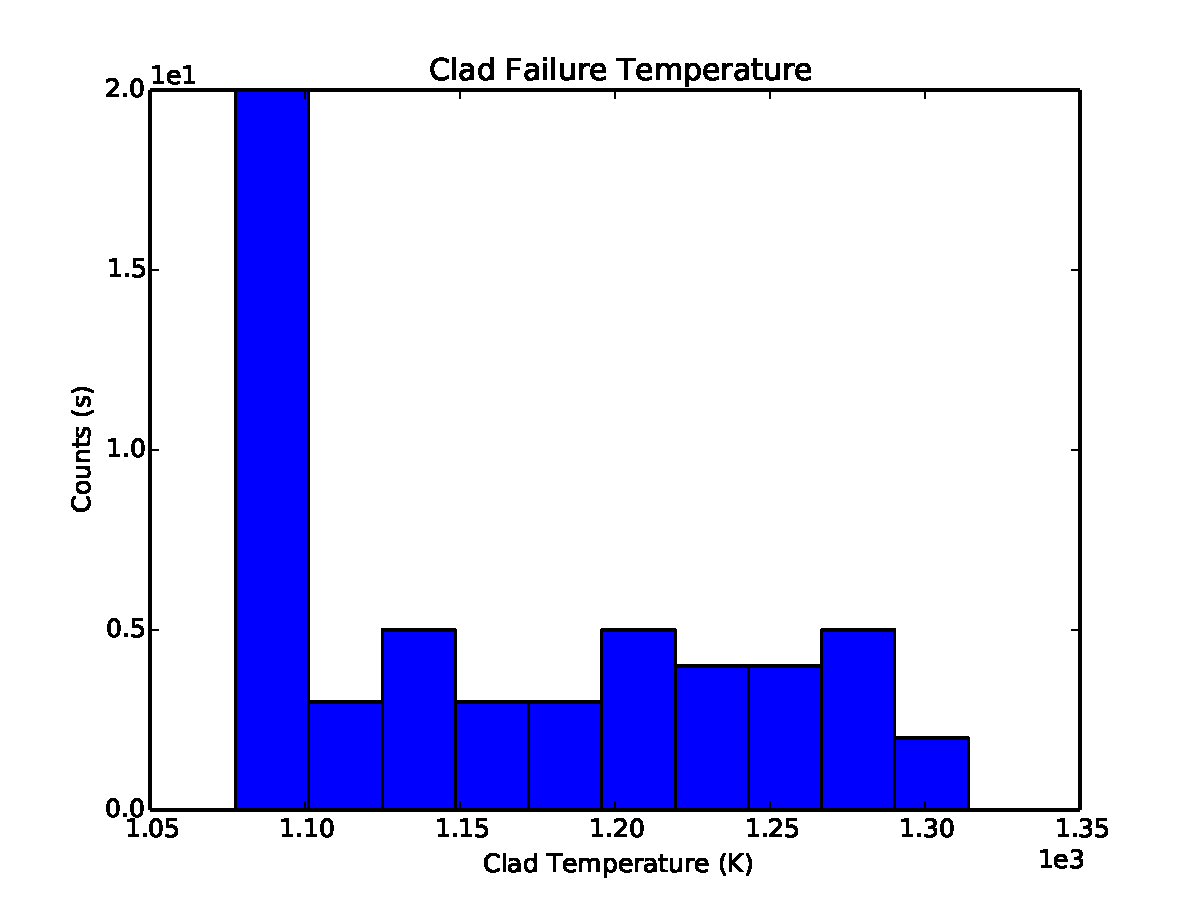
\includegraphics[width=9cm]{figures/HistogramSampledVarCladFailureDET_histogram.pdf}
   %\caption{Histogram of Clad Failure Temperature (DET).}
   %\label{fig:DETpbClad}
 \end{minipage}
 \ \hspace{2mm} \hspace{3mm} \
 \begin{minipage}[b]{8.5cm}
   \centering
   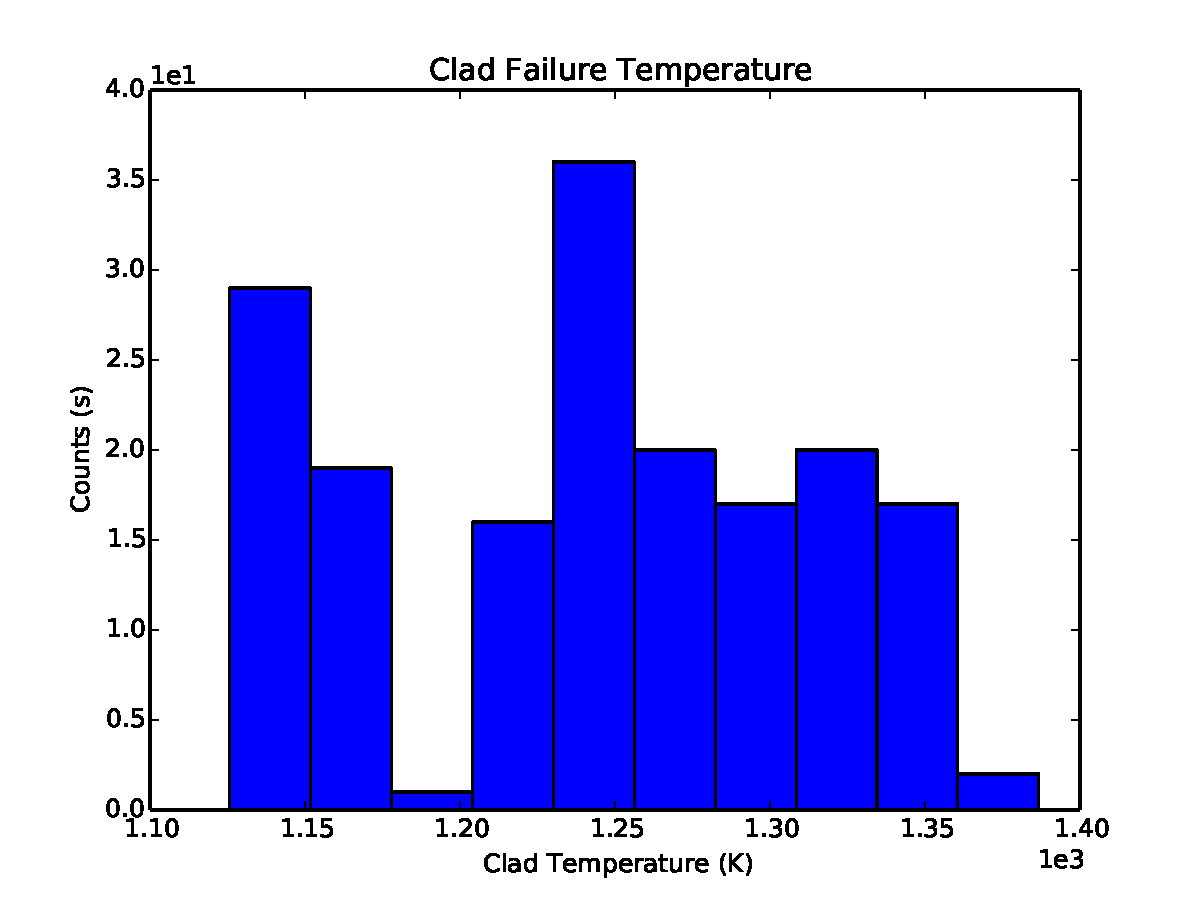
\includegraphics[width=9cm]{figures/HistogramSampledVarCladFailureADET_histogram.pdf}
   %\caption{Histogram of Clad Failure Temperature (ADET).}
   %\label{fig:DETpbHead}
 \end{minipage}
\caption{Histogram of Clad Failure Temperature for DET (Left) and ADET (Right)}
\label{fig:SampledTEMP}
\end{figure}
%%% SAMPLED TEMPERATURE

%%% SAMPLED PARAMETERS COLLAPSED
\begin{figure}[h]
 \begin{minipage}[b]{8.5cm}
   \centering
   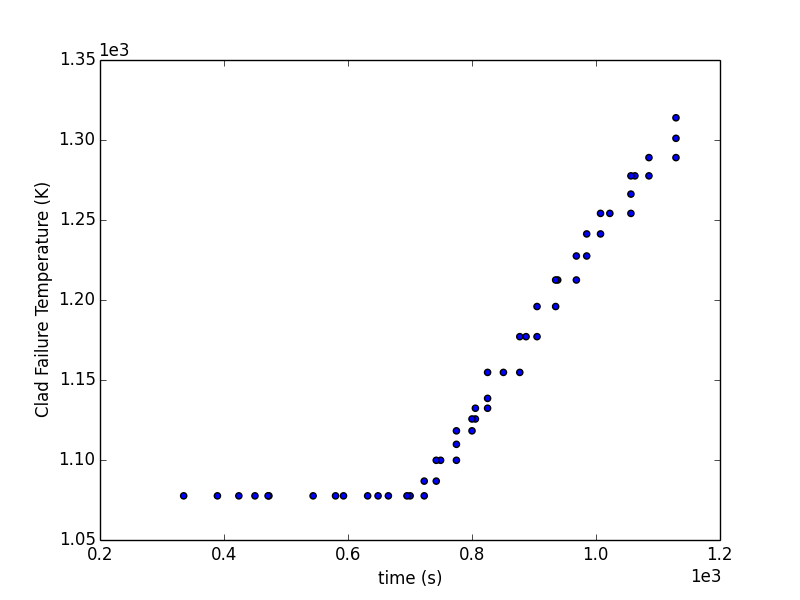
\includegraphics[width=9cm]{figures/sampledcollapsed_det.png}
   %\caption{Histogram of Clad Failure Temperature (DET).}
   %\label{fig:DETpbClad}
 \end{minipage}
 \ \hspace{2mm} \hspace{3mm} \
 \begin{minipage}[b]{8.5cm}
   \centering
   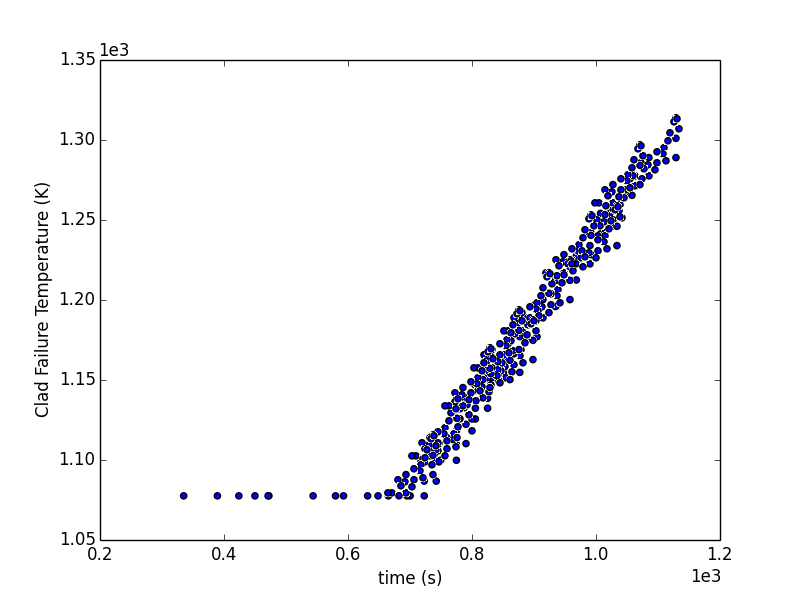
\includegraphics[width=9cm]{figures/sampledcollapsed_adaptivedet.png}
   %\caption{Histogram of Clad Failure Temperature (ADET).}
   %\label{fig:DETpbHead}
 \end{minipage}
\caption{Sampled Parameters (Collapsing Recovery times) for DET (Left) and ADET (Right)}
\label{fig:SampledCollapsed}
\end{figure}
%%% SAMPLED PARAMETERS COLLAPSED
%%%%%%%%%%%%%%% LIMIT SURFACE
\begin{figure}[h]
  \centering
     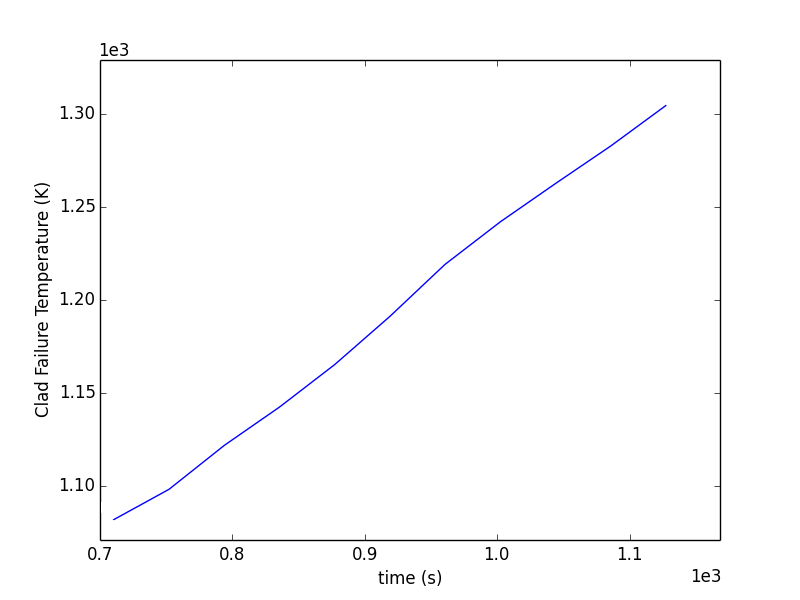
\includegraphics[width=1\textwidth]{figures/LS-2D-DET.png}
  \caption{Limit Surface DET/ADET.}
   \label{fig:LS_DETADET}
\end{figure}


